%Publication version
\documentclass[aps,twocolumn,prd,superscriptaddress,showpacs,nofootinbib,fixfloat]{revtex4}
%Draft version
%\documentclass[aps,prd,superscriptaddress,showpacs]{revtex4}
%\usepackage{doublespace}
\usepackage{graphicx}
\usepackage{dcolumn}
\usepackage{bm}
\usepackage{natbib}

%\topmargin+1cm

% Journals
\newcommand{\aaps}{{Astron.~Astrophys.~Supp.}}
\newcommand{\physrep}{{Physics~Reports}}
\newcommand{\araa}{{Annu.~Rev.~Astron.~Astrophys.}}
\newcommand{\aap}{{Astron.~Astrophys.}}
\newcommand{\apjl}{{Astrophys.~J.~Lett.}}
\newcommand{\apjs}{{Astrophys.~J.~Supp.}}
\newcommand{\aj}{{Astron.~J.}}
\newcommand{\mnras}{{Mon.~Not.~R.~Astron.~Soc.}}

% Making life easier
\newcommand{\be}{\begin{equation}}
\newcommand{\ee}{\end{equation}}
\newcommand{\bea}{\begin{eqnarray}}
\newcommand{\eea}{\end{eqnarray}}
\newcommand{\backten}{\!\!\!\!\!\!\!\!\!\!}

% useful symbols
\newcommand{\nhat}{\hat{\bf n}}
\newcommand{\kvec}{{\bf k}}
\newcommand{\edm}{\epsilon_{dm}}
\newcommand{\edmnow}{\epsilon_{dm,0}}
\newcommand{\sv}{\langle\sigma_Av\rangle}
\newcommand{\khat}{\hat{\bf k}}

% Fermi is usually italicized - use \Fermi\ for space after word
\newcommand{\Fermi}{{\slshape Fermi}}

% math functions, units
\newcommand{\Mpc}{{\rm ~Mpc}}
\newcommand{\sech}{{\rm ~sech~}}
\newcommand{\Tr}{{\rm ~Tr~}}
\newcommand{\threej}[6]{{\left( \begin{array}{ccc} #1 & #2 & #3 \\ #4 & 
   #5 & #6 \end{array} \right)}}

% Doug's units
\newcommand{\s}{{\rm ~s}}
\newcommand{\kms}{{\rm ~km/s}}
\newcommand{\g}{{\rm ~g}}
\newcommand{\cm}{{\rm ~cm}}
\newcommand{\km}{{\rm ~km}}
\newcommand{\mm}{{\rm ~mm}}
\newcommand{\mJy}{{\rm ~mJy}}
\newcommand{\Jy}{{\rm ~Jy}}
\newcommand{\MJy}{{\rm ~MJy}}
\newcommand{\MJypSr}{{\rm ~MJy~sr^{-1}}}
\newcommand{\JypSr}{{\rm ~Jy~sr^{-1}}}
\newcommand{\Hz}{{\rm ~Hz}}
\newcommand{\kHz}{{\rm ~kHz}}
\newcommand{\MHz}{{\rm ~MHz}}
\newcommand{\GHz}{{\rm ~GHz}}
\newcommand{\K}{{\rm ~K}}
\newcommand{\mK}{\rm ~mK}
\newcommand{\microK}{\mu{\rm K}}
\newcommand{\eV}{{\rm ~eV}}
\newcommand{\eVs}{{\rm ~eV/s}}
\newcommand{\keV}{{\rm ~keV}}
\newcommand{\MeV}{{\rm ~MeV}}
\newcommand{\GeV}{{\rm ~GeV}}
\newcommand{\TeV}{{\rm ~TeV}}
\newcommand{\pc}{{\rm ~pc}}
\newcommand{\kpc}{{\rm ~kpc}}
%\newcommand{\Mpc}{{\rm ~Mpc}}
\newcommand{\erg}{{\rm ~erg}}
\newcommand{\degree}{^{\rm o}}
\newcommand{\sigmav}{\langle\sigma_Av\rangle}
\newcommand{\zrock}{$Z_{\rm rock}$}
\def\la{\vcenter{\hbox{$<$}\offinterlineskip\hbox{$\sim$}}}
\def\ga{\vcenter{\hbox{$>$}\offinterlineskip\hbox{$\sim$}}}


% Necessary for appendices
\newcommand{\lmax}{{l_{\rm max}}}
\newcommand{\lmaxtwo}{{l_{\rm max}^2}}
\newcommand{\lmaxthree}{{l_{\rm max}^3}}


\newcommand\dpf[1]{{\bf (DPF: #1)}}

\begin{document}


\title{Is the 130 GeV Line Real? \\
  A Search for Systematics in the Fermi-LAT Earth Limb Data}

\author{Douglas P. Finkbeiner}
%\email{dfinkbeiner@cfa.harvard.edu}
\affiliation{Institute for Theory and Computation,
  Harvard-Smithsonian Center for Astrophysics, 
  60 Garden Street, MS-51, Cambridge, MA 02138 USA} 
\affiliation{Center for the Fundamental Laws of Nature,
  Physics Department, 
  Harvard University, 
  Cambridge, MA 02138 USA}

\author{Meng Su}
\affiliation{Institute for Theory and Computation,
  Harvard-Smithsonian Center for Astrophysics, 
  60 Garden Street, MS-51, Cambridge, MA 02138 USA} 

\author{Christoph Weniger}
\affiliation{Max-Planck-Institut f\"ur Physik, 
  F\"ohringer Ring 6, 
  80805 M\"unchen, Germany}

\begin{abstract} Our recent claims of a Galactic center feature in Fermi/LAT
  data at approximately 130 GeV have prompted an avalanche of papers proposing
  explanations ranging from dark matter annihilation to exotic pulsar winds.
  Because of the importance of such interpretations for physics and
  astrophysics, the threshold for discovery is unusually high.  This requires
  not only additional data, but a thorough investigation of possible LAT
  systematics.  While we do not have access to the details of each event
  reconstruction, we do have information about each event from the public
  event lists and spacecraft parameter files.  These data allow us to search
  for suspicious trends that could indicate a spurious signal.  In particular,
  the Earth limb photons provide a smooth reference spectrum for null tests.
  We examine these events and find a marginally significant 130 GeV feature in
  a small subset of the data.  This raises concerns about the 130 GeV Galactic
  center feature, even though we can think of no plausible model of
  instrumental behavior that connects the two.  A modest amount of additional
  limb data would tell us if the limb feature is a statistical fluke.  If the
  limb feature persists, it raises serious concerns about the Pass 7
  processing of $E > 100$ GeV events.
\end{abstract}

\pacs{}

\maketitle

\section{Introduction}
The search for dark matter takes many forms:  exploration of its astrophysical
properties, direct detection in underground labs, and even collider signatures
of WIMPs or related particles.  (cite reviews).   Etc. 

A gamma-ray line is a long-sought smoking gun for WIMP annihilation. 

We were not optimistic, because the branching ratio to lines is loop
suppressed, and one would have expected to see a continuum first in e.g. MSSM
models.  However, there are other models (e.g. MiDM) that allow high line to
continuum ratios.  In this work, we drop all theoretical prejudice and simply
ask if there is a line in the Galactic center spectrum. 

The first claim of a line around 130 GeV emerged from the work of Weniger
(cite), which grew out of an earlier search for other hard photon signals from
annihilations (Bringmann).  Weniger focused on spectral fitting to photon
events in regions of interest designed to maximize S/N.  He found a XXX sigma
signal at 130 GeV. 

Subsequent work by Su \& Finkbeiner approached the problem with template
fitting, assuming various profiles (Einasto, NFW, Gaussian) for the DM
distribution.  If the template is correct, this should allow extraction of the
DM signal with higher S/N.   This work found XXX sigma for an Einasto profile
centered $1.5\degree$ W of the Galactic center, and also suggest that there
may be two lines, at about 111 and 129 GeV.  The lower energy is tantalizing
because it matches the expected energy of a $Z\gamma$ line if the higher
energy is the $\gamma\gamma$ line. 

These papers have provoked theorists to try to reconcile the observations with
a number of theories (cite dozens of papers).  But all of this work depends on
the question:

(What was the question?)


\section{The 130 GeV excess}

\subsection{Standard survey strategy and definitions}

\begin{figure}[h]
  \begin{center}
    % \includegraphics{<+file+>}
    \fbox{\Huge Figure}
  \end{center}
  \caption{Phi/theta distribution of all events}
  \label{fig:phiThetaDist}
\end{figure}

In standard survey mode, the LAT points at zenith angle \zrock\ north of the
zenith on one orbit and \zrock\ south of the zenith on the next.  \zrock\ was
$35\degree$ early in the survey, but was changed to $50\degree$ in 2009 for
better thermal management of the downward-facing battery radiator.  This
rocking profile, combined with the precession of the orbit every 55 days,
allows the LAT to cover the whole sky every two orbits with approximately
uniform coverage.  This survey mode is only occasionally interrupted for
pointed observations of targets of opportunity (ToOs). 

\textbf{Define all parameters, $\theta$, $\phi$, $z$, $x-y-z$ coordinates etc}

\begin{table*}
\begin{center}
  \begin{tabular}{l|rr|l}
    \hline
    Parameter & & Range &  Description\\
    name      & min & max &            \\
    \hline
    $\theta$ &    0 &  $\sim80$ & Polar coordinate (instrument frame) \\
    $\phi$   &    0 &       360 & Azimuthal coordinate (instrument frame) \\
    $Z$      &    0 & $\sim113$ & Zenith angle (horizon at $Z=113\degree$) \\
    \zrock\  & -110 & 110 & Rocking angle (boresight angle N of zenith \\
    $\ell$   &    0 & 360 & Galactic longitude \\
    $b$      &  -90 &  90 & Galactic latitude \\
    $\psi$   &    0 & 180 & Angle to Galactic center.  $\cos\psi=\cos\ell\cos b$ \\
    \hline
  \end{tabular}
  \caption{Parameter definitions}
  \label{tab:eventRatios}
\end{center}
\end{table*}




\textbf{Discuss standard event selection used throughout}

\subsection{Peculiarities of the Galactic center observation}
The fact that the dominant 130 GeV line signal is near the Galactic center
raises a number of concerns.  The GC is near the ecliptic ($\beta \approx
-5\degree$) and may be observed in a restricted range of angles in instrument
coordinates $(\theta, \phi)$ when the Sun passes near it.  Also, the gamma-ray
flux at the GC is somewhat brighter and has a harder spectrum than neighboring
regions.  We consider whether these facts could exacerbate any systematic
errors in the LAT data to produce a spurious signal.

{\bf note: The subsection titles could relate to the hypothesis being tested.
For example: ``Hypothesis: the GC observations have a restricted range of
incidence angles on the instrument'' or ``Hypothesis: The Galactic center is
bright, so instrumental artifacts are more significant there'' and so on.
Just to be exceedingly clear about what we are testing.}

\subsubsection{Is the Galactic center observed at peculiar incidence angles?}

\begin{figure*}
  \centering
  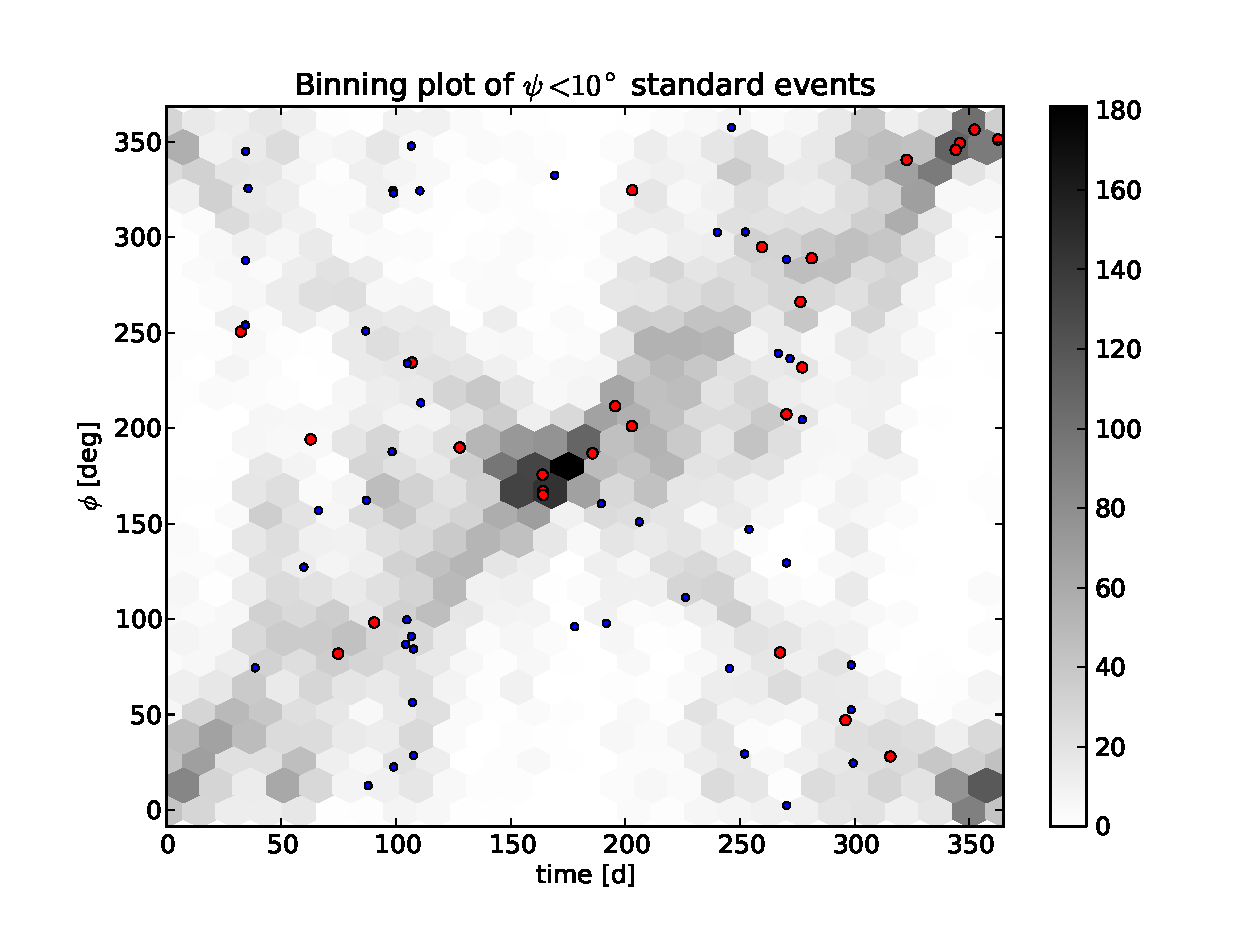
\includegraphics[width=0.44\textwidth]{plots/TIME_PHI.eps}
  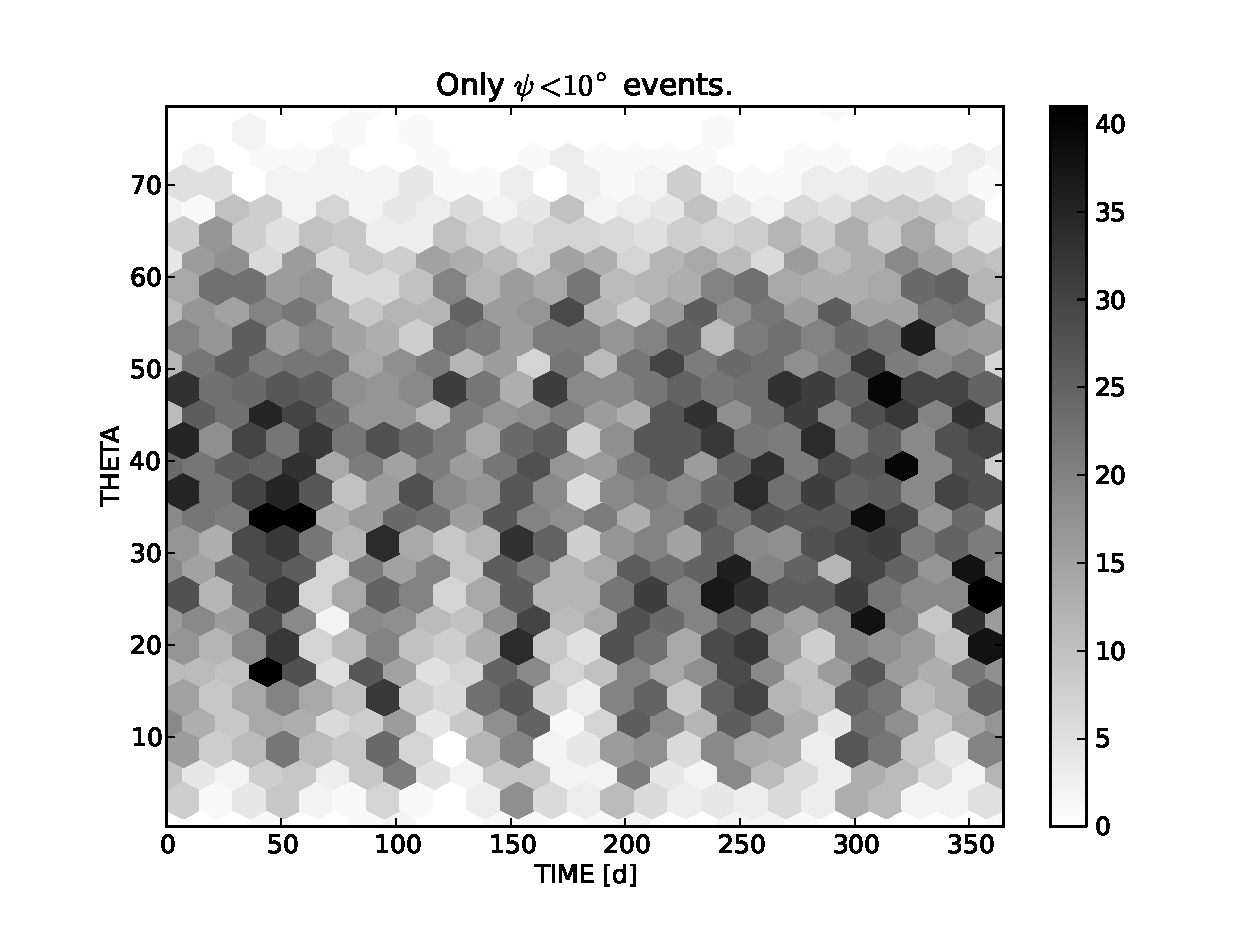
\includegraphics[width=0.44\textwidth]{plots/TIME_THETA.eps}
  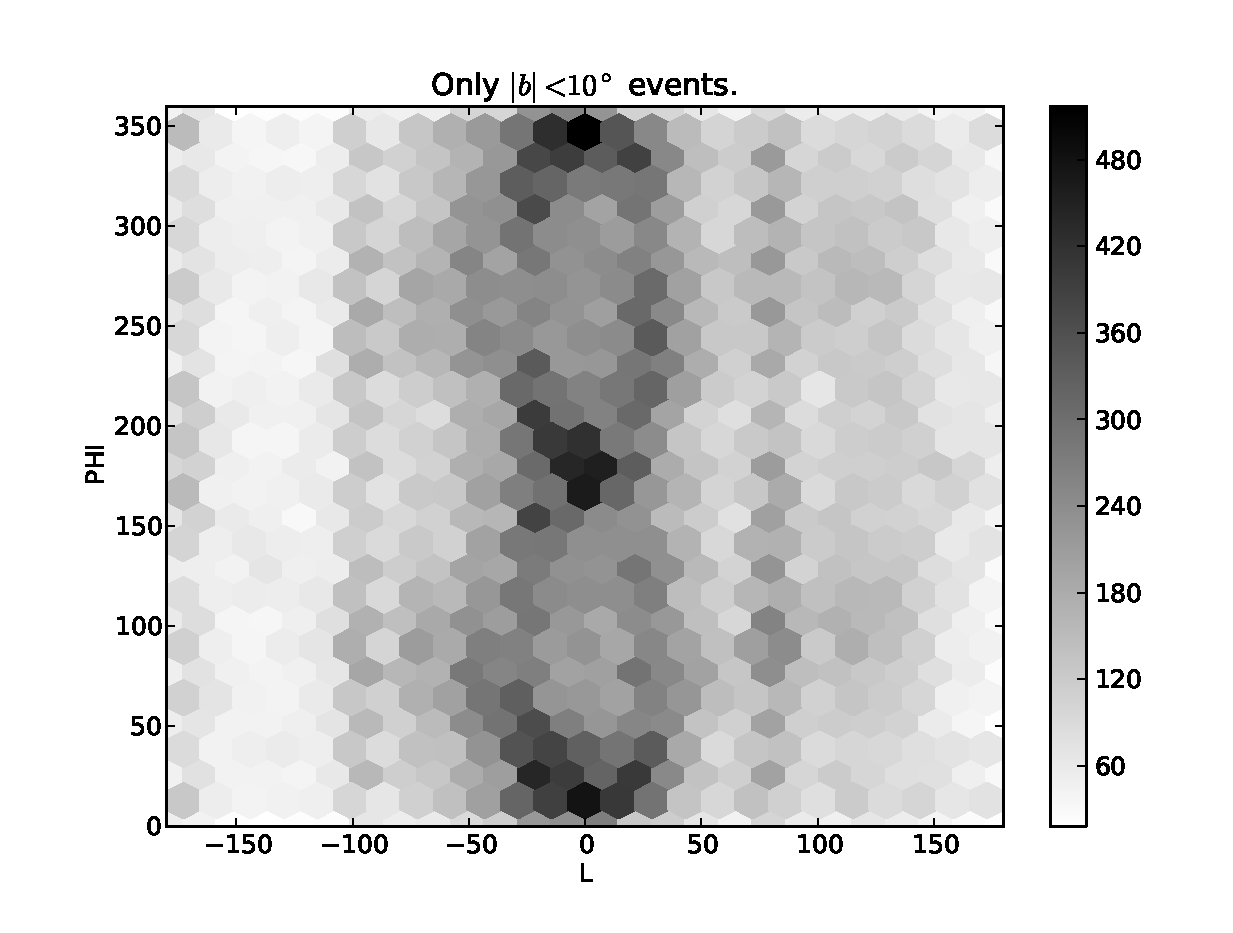
\includegraphics[width=0.44\textwidth]{plots/L_PHI.eps}
  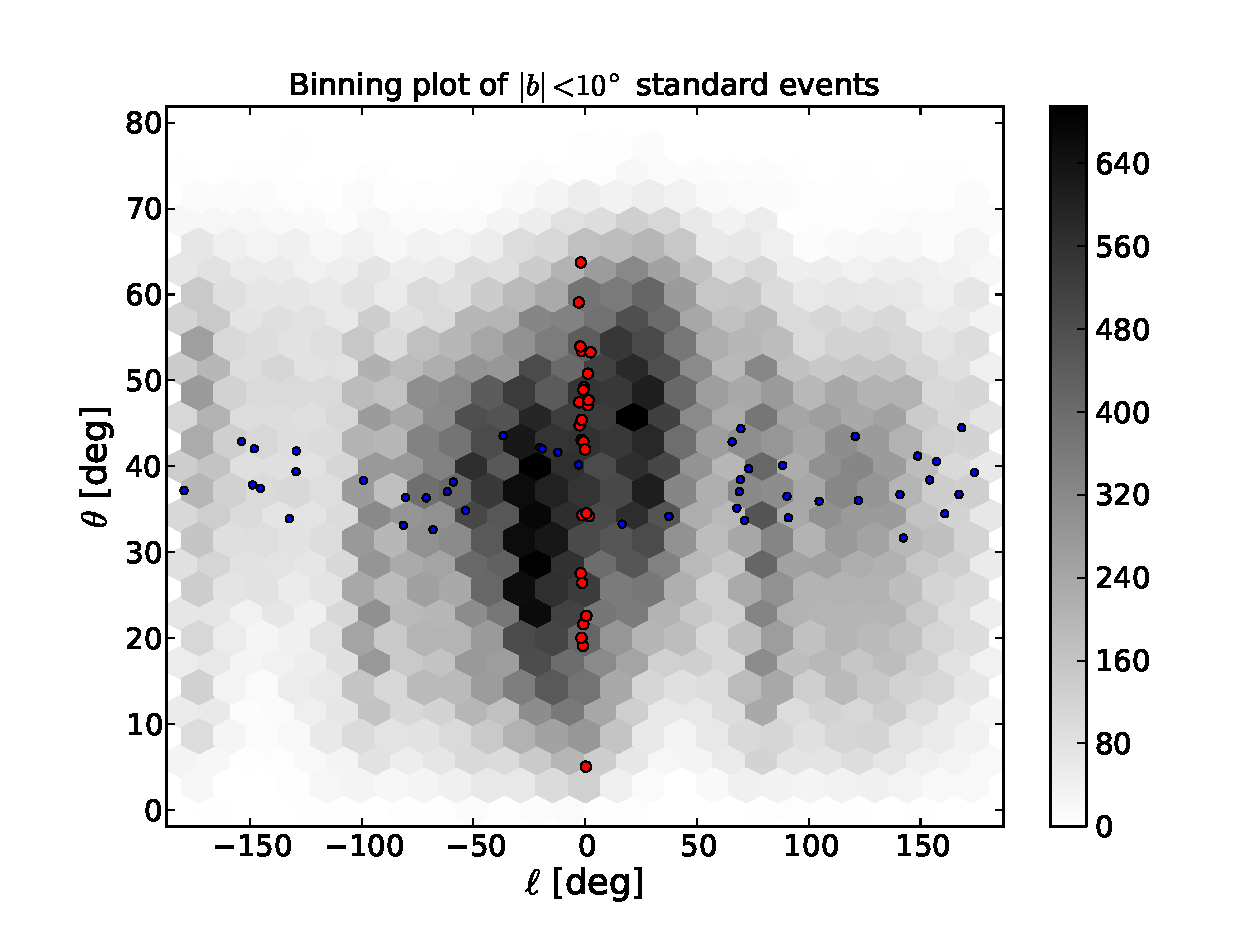
\includegraphics[width=0.44\textwidth]{plots/L_THETA.eps}
  \caption{\emph{Upper panels:} PHI (left panel) and THETA (right panel)
  distribution of GC events as function of time modulo one year (with Jan 1st
  at the origin). In Dec (Jun) the Sun passes near the Galactic center
  (anti-center).  In these periods, most events are observed at $\phi\approx
  0^\circ$ ($\phi\approx 180^\circ$), since the LAT $x-z$ plane is
  determined by the Sun to keep the solar panels oriented. \emph{Lower panels:}
  PHI (left panel) and THETA (right panel) distribution of events along the
  galactic disk. Close to the GC, the distribution becomes significantly
  bimodal.}
  \label{fig:time_phi}
\end{figure*}

\begin{figure}
\centering
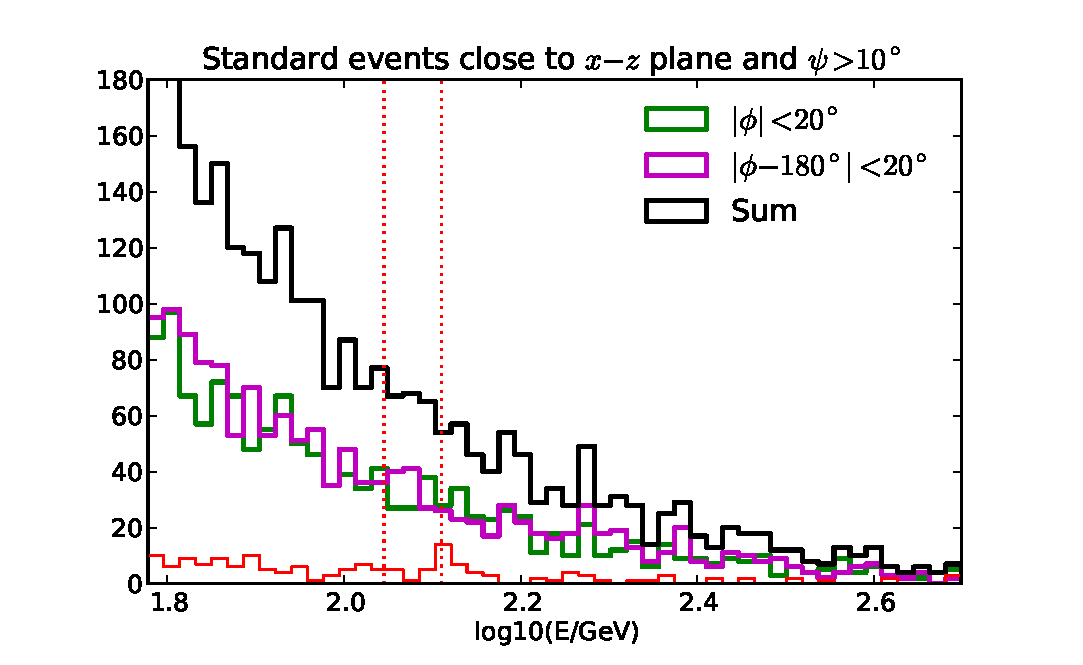
\includegraphics[width=1.0\linewidth]{plots/phi_energy.eps}
\caption{Energy distribution of all-sky events with incidence angles close to
the LAT $x-z$ plane (perpendicular to the solar panels). The red dotted lines
indicates 111 and 130 GeV.}
\label{fig:spectrum_phi}
\end{figure}

In case the Galactic center is predominantly observed under specific angles in
LAT instrumental coordinates, associated instrumental problems could be
projected onto the Galactic center simply for geometrical reasons. The sky
coverage of Fermi at various incidence angles is usually approximately uniform,
but this is not necessarily the case for the Galactic center.  In late December
(June), the angular distance between the Sun and the Galactic center
(anti-center) reduces to about $5^\circ$.  Since Fermi keeps the solar panels
aligned to the Sun, this leads to an increase of Galactic center events at
instrument azimuth angles of $\phi\approx 0^\circ$ ($\phi\approx 180^\circ$).
This behaviour is clearly visible in the upper left panel of Fig.~\ref{fig:time_phi}, where we show
the $\phi$ distribution of $>10\GeV$ events from the Galactic center as
a function of time (modulo one year).  The $\theta$ distribution in the upper
right panel shows the precession pattern of 55 days \textbf{(check!)}.
Integrated over time, the $\phi$ and $\theta$ distributions look like in the
lower panels of Fig.~\ref{fig:time_phi}.

It is tempting to relate the locality of the 130 GeV excess in the Galactic
plane to this inhomogeneous $\phi$ distribution. A simple check (and
rejection) of this idea goes as follows: We select standard events from the
full sky (excluding $\psi < 10^\circ$) in the range close to $\phi\approx
0^\circ\ \text{mod}\ 180^\circ$. The total number of these events is about 10
times larger than the number of Galactic center events (here $\psi<3^\circ$)
at all $\phi$; an anomaly in the event reconstruction under these $\phi$
angles should appear in this data sample with high significance. However, the
energy distribution shown in Fig.~\ref{fig:spectrum_phi} shows no significant
feature at 111 or 130 GeV.

\subsubsection{Is the Galactic center distinct due to its high flux?} Besides
the Galactic center ($\psi<3^\circ$) with $\approx80$ events above 100 GeV, a
few other bright regions exist.  The most important are the
Earth limb ($\approx2800$ events at $Z>110^\circ$ and \emph{all} impact
angles) and the Galactic bulge ($\approx640$ events at
$3^\circ<|\ell|\lesssim30^\circ$, $|b|<2^\circ$ \textbf{(does this definition
make sense? -- I would call this the inner Galactic plane - DPF)}).\footnote{In the vicinity ($<0.5^\circ$) of the bright point
sources Vela and Geminga only two $>100\GeV$ events were measured.} These
targets provide a large number of high energy photons that can be used to
check for systematic artifacts in the energy spectra. The largest test sample,
however, with events at all impact angles, is simply the full set of all
standard events, excluding only the Galactic center $\psi<10^\circ$ ($\approx
4300$ events). For all these targets, we show the energy distribution in
Fig.~\ref{fig:target_spectra}.  None of the regions exhibit an
$\mathcal{O}(1)$ excess at 130 GeV as observed in the Galactic center.

\begin{figure}
\centering
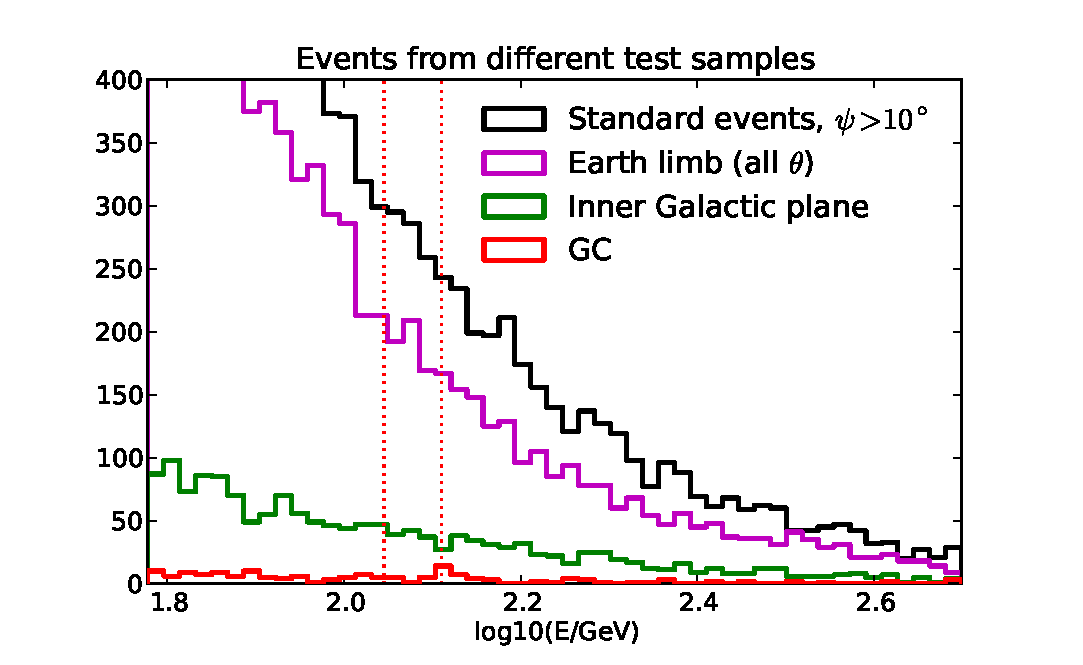
\includegraphics[width=1.0\linewidth]{plots/target_spectra.eps}
\caption{Energy distribution in various bright regions.  None of them show the
  excess events around 130 GeV seen in the Galactic center.  \textbf{(improve
plot)}.}
\label{fig:target_spectra}
\end{figure}

\subsubsection{Are energy spectra in the Galactic center particularly hard?}

One concern is that the Galactic center might harbour an unusually large
number of sources with very hard spectra. If these high energy photons are
occasionally mis-reconstructed with energies close to 130 GeV, this could
produce a line feature in the data that would dominantly show up at the
Galactic center. As a simple check for this possibility, we calculated the
ratio of events above $300\GeV$ (and up to $500\GeV$) to events above
$100\GeV$ in different regions of the sky. The results are shown in
Tab.~\ref{tab:eventRatios}.  The Galactic center does not harbour significantly
more high energy events than other regions of the sky, none of which
exhibit a feature at 130 GeV (see Fig.~\ref{fig:target_spectra}). 

About 10--15 events contribute to the line feature seen at the GC. Assuming
that fluxes are not harder than $dN/dE \propto E^{-2.6}$, most of these events
would
have to come from energies below $300\GeV$, since there would be not enough
events above this energy to make up the 130 GeV excess even if \emph{all} of
them were incorrectly mapped to 130 GeV. 

\begin{table}
  \begin{tabular}{lrr}
    \hline
    Region & $\frac{N(>100\GeV)}{N(>30\GeV)}$ & $\frac{N(>300\GeV)}{N(>100\GeV)}$\\
    \hline
    $\psi<3^\circ$ & 17.6\% & 9.2\% \\
    $z>110^\circ$  & 10.3\% & 9.2\% \\
    $3^\circ < |\ell| < 30^\circ,\ |b|<2^\circ$ & 16.9\% & 10.1\% \\
    $\psi>10^\circ$ & 13.2\% & 9.3\% \\
    \hline
  \end{tabular}
  \caption{Event ratios in different regions of the sky}
  \label{tab:eventRatios}
\end{table}

\subsection{Peculiarities of the instrument}

\subsubsection{Indications for artifacts at different incidence angles?}
In Fig.~\ref{fig:polarPlotsAll}, we show the statistical significance for a
line when scanning over $(\theta, \phi)$ subsamples of the full-sky data.

\textbf{Add more details}

\begin{figure*}[p]
  \centering
  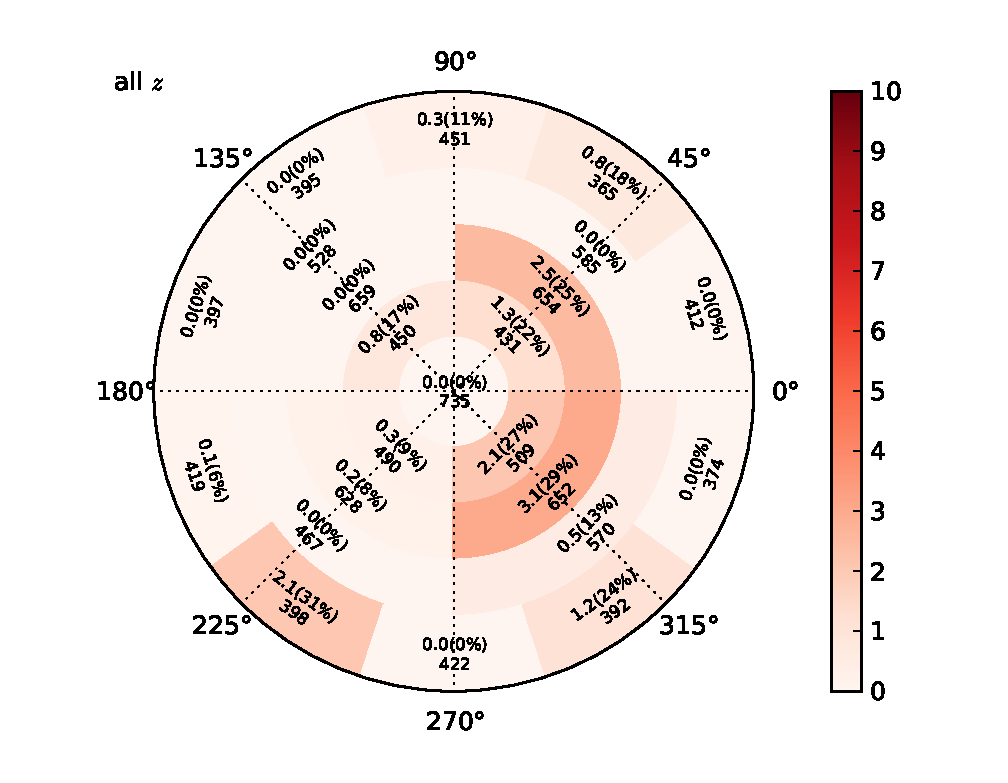
\includegraphics[width=0.45\textwidth]{plots/polar_all.eps}
  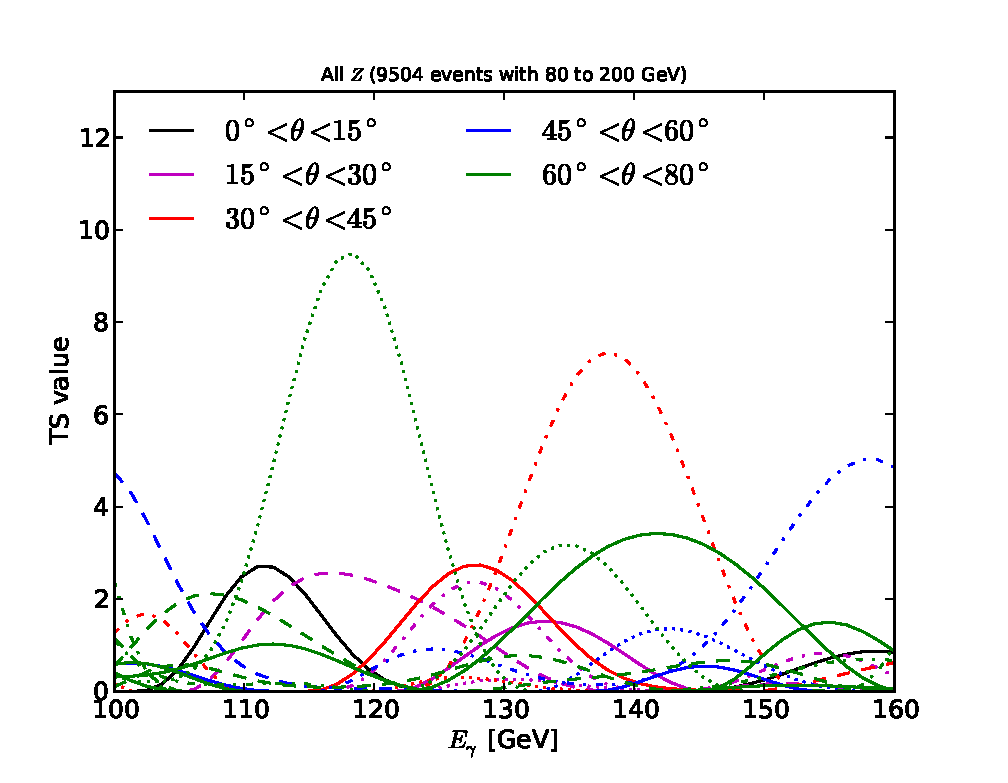
\includegraphics[width=0.40\textwidth]{plots/scan_all.eps}
  \includegraphics[width=0.45\textwidth]{plots/polar_z.GT.110.eps}
  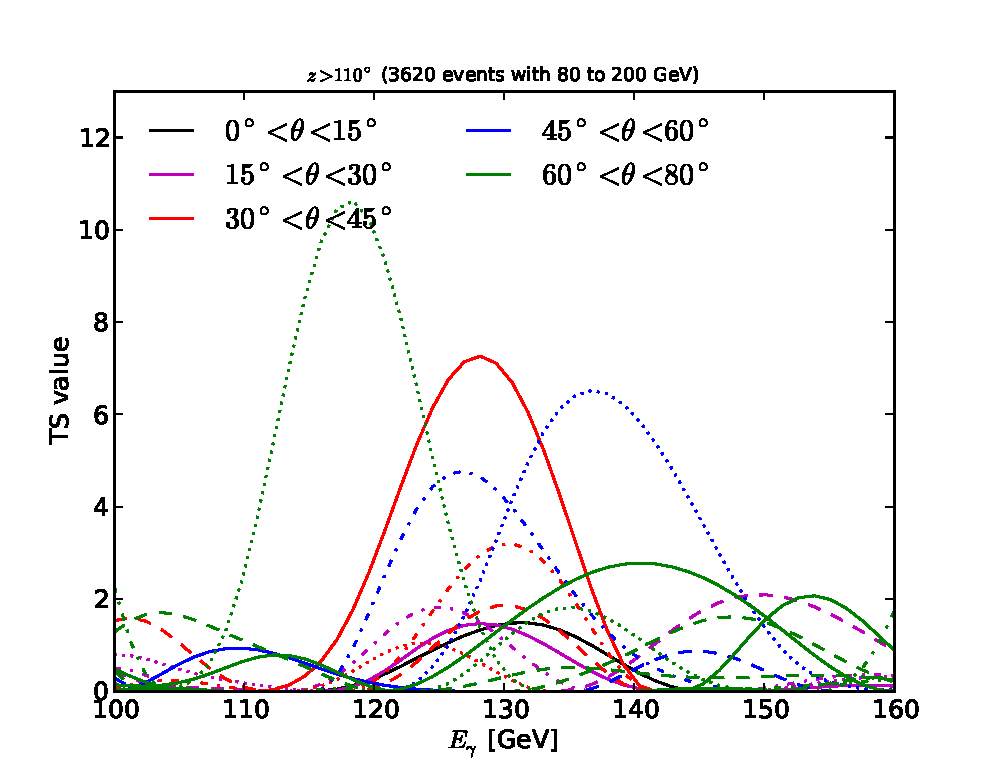
\includegraphics[width=0.40\textwidth]{plots/scan_z.GT.110.eps}
  \includegraphics[width=0.45\textwidth]{plots/polar_z.LE.100.eps}
  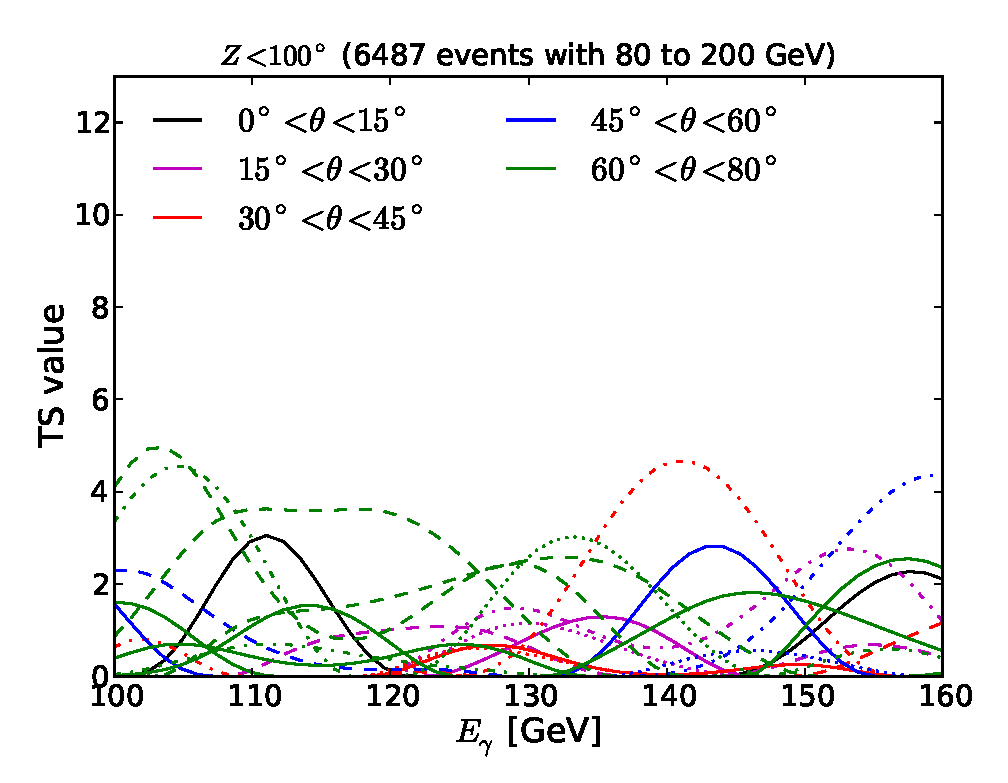
\includegraphics[width=0.40\textwidth]{plots/scan_z.LE.100.eps}
  \caption{\emph{Left panels:} Significance for a 130 GeV line-like excess in different parts of
  the $\theta$-$\phi$ plane (for $\theta=0$--$80^\circ$). The three numbers
  show the TS value for the presence of a 130 GeV line, the
  signal-to-background ratio and the number of events above $80\GeV$ inside
  the considered $\theta$-$\phi$ region. \emph{Right panels:} The significance
  for a $E_\gamma$ line-like excess for the same $\theta$-$\phi$ regions.
  \textbf{(add 130 GeV to figure)}.}
  \label{fig:polarPlotsAll}
\end{figure*}

\subsubsection{Indications for a bad event reconstruction?}
There could be indications, but there are not. See Fig.~\ref{fig:CTBquality}.
\text

\begin{figure*}
  \centering
  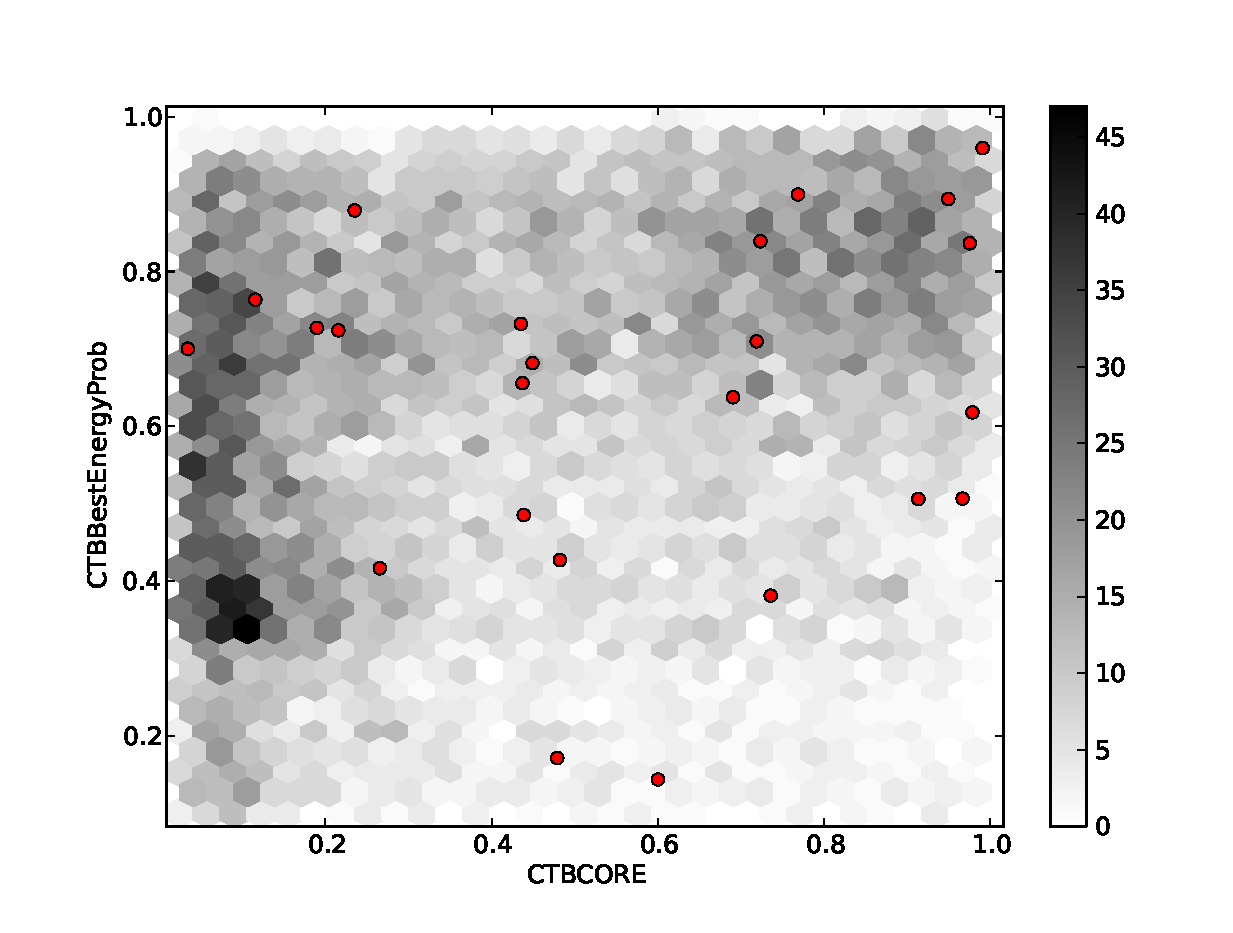
\includegraphics[width=0.48\linewidth]{plots/CTBCORE_CTBBestEnergyProb.eps}
  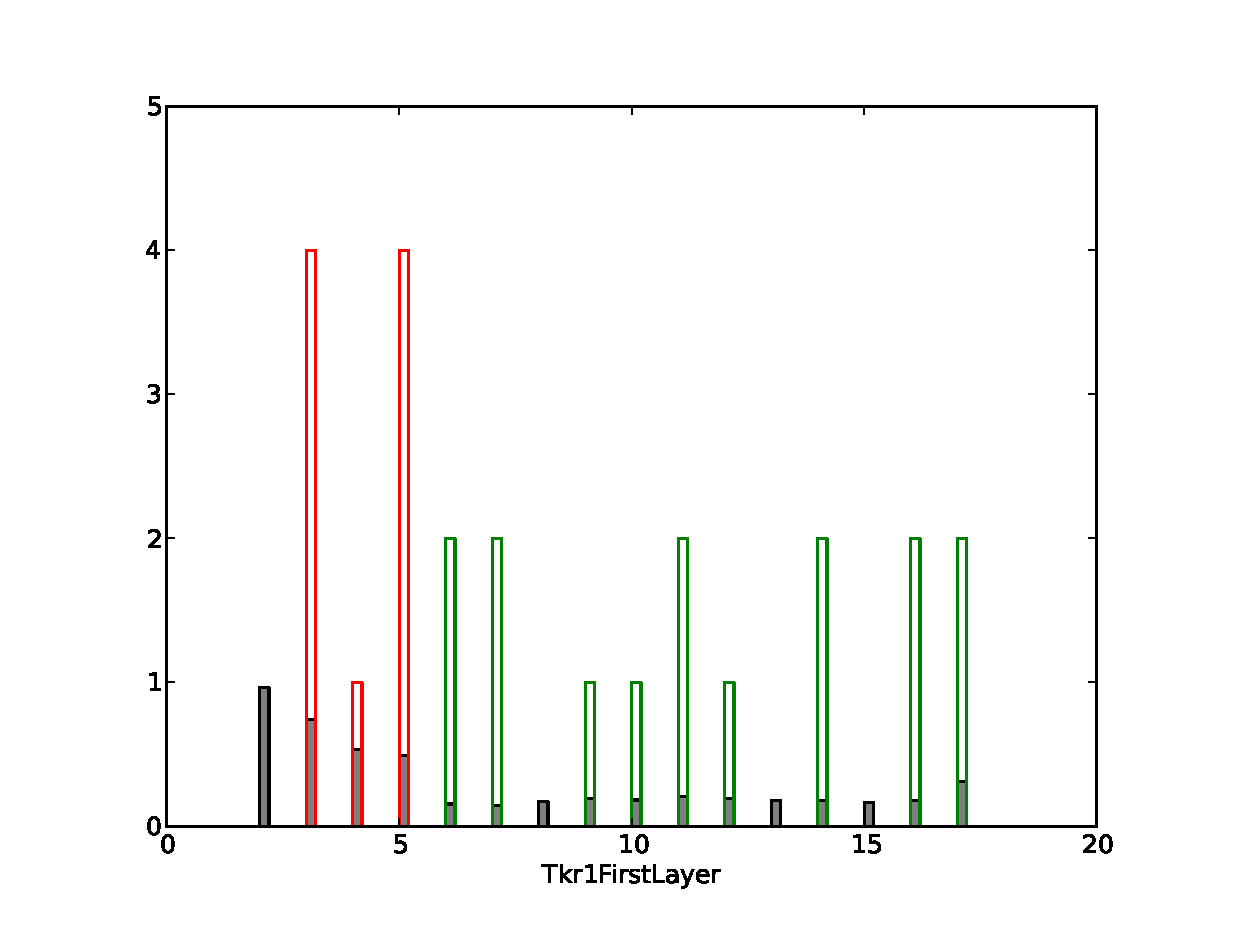
\includegraphics[width=0.48\linewidth]{plots/Tkr1FirstLayer.eps}
  \caption{\emph{Left panel:} Distribution of CTBCORE (the probability that
  the direction estimate is good) and CTBBestEnergyProb (the probability that
  the best energy chosen from the two energy estimators is correct) for GC
  events (in red), compared to average distribution for $>50$ GeV events.
  \emph{Right panel}: First tracker layer to show evidence of a particle hit
  for the best track reconstruction. Tracker layers are 0-17 where 0 is
  closest to the calorimeter, and 6-17 (2-5) corresponds to front-
  (back-)converting events (tracker layers 0 and 1 come without conversion
  foils). The gray bars show the distribution averaged over all $>100$ GeV
  events, the green/red bars show the distribution for the GC line.}
  \label{fig:CTBquality}
\end{figure*}

\clearpage
\section{Earth limb photons}
At an altitude $a$, the geometric (unrefracted) horizon is at zenith angle
\be
Z_{\rm hor} = \cos^{-1}\left(\frac{R_\oplus}{R_\oplus+a}\right)+90\degree
\ee
The Fermi orbit is nearly circular with $535 < a < 564$, yielding $Z_{\rm
  hor}$ in the 112.7$\degree$ to 113.3$\degree$ range, with the tangent point
some 2400 km distant.  At this distance, the 90 km height of the atmosphere
subtends about $2\degree$, or roughly $111 < Z < 113$.  

At lower zenith angles ($Z \la 105\degree$) Fermi observes the sky with very
little background from the limb.  The incidence angle on the detector,
$\theta$, is defined such that $\theta=0$ corresponds to the ``boresight.''
For \zrock = $50\degree$, the limb photons are typically at $\theta >
60\degree$ (See figure \ref{fig:theta-E}.

We begin by examining the limb events and finding a bump at 130 GeV in a
subsample of these events.  We consider two hypothesis for the origin of the
bump: that the events come from far away in energy, or the more subtle
possibility that an energy mapping error could redistribute in energy, making
a spectral feature.  We then explore the various parameters of the GC line
events and the limb bump events. 

The continual cosmic-ray cascades in the Earth's atmosphere produce gamma rays
with $dN/dE \sim E^{-2.6}$.  (check this???)  These atmospheric gammas are
referred to as ``Earth limb photons'' or sometimes as ``albedo photons.''
These photons provide a convenient reference sample to search for systematics
in the LAT data.  Because the limb photons result from atmospheric cascades,
they are produced by interactions in a highly boosted frame, and cannot
contain line emission. 

\begin{figure}[p]
  \centering
  \includegraphics[width=1.0\linewidth]{plots/theta-E.ps}
  \caption{Incidence angle $\theta$ vs. log $E$ for $Z > 105\degree$.  A blue
  box indicates the region $30\degree < \theta < 45\degree$ and 125 GeV $< E
  <$ 140 GeV, where an excess of events appear.  The vast majority of limb
  events are at $\theta > 60\degree$ because the telescope seldom points more
  than $50\degree$ from zenith, and the limb events are mostly at
  $Z>110\degree$.}
  \label{fig:theta-E}
\end{figure}

\begin{figure}[p]
  \centering
  \includegraphics[width=1.0\linewidth]{plots/Ehist-all.ps}
  \caption{Histogram of limb $(Z>105\degree)$ events vs. log($E$) for various
  ranges of $\theta$. The position of the 130 GeV line is indicated (red
  dotted line).  Note the excess in the $30\degree < \theta < 45\degree$ bin,
  which contains about 5\% of the limb events.}
  \label{fig:Ehist-all}
\end{figure}

\begin{figure*}[p]
  \centering
  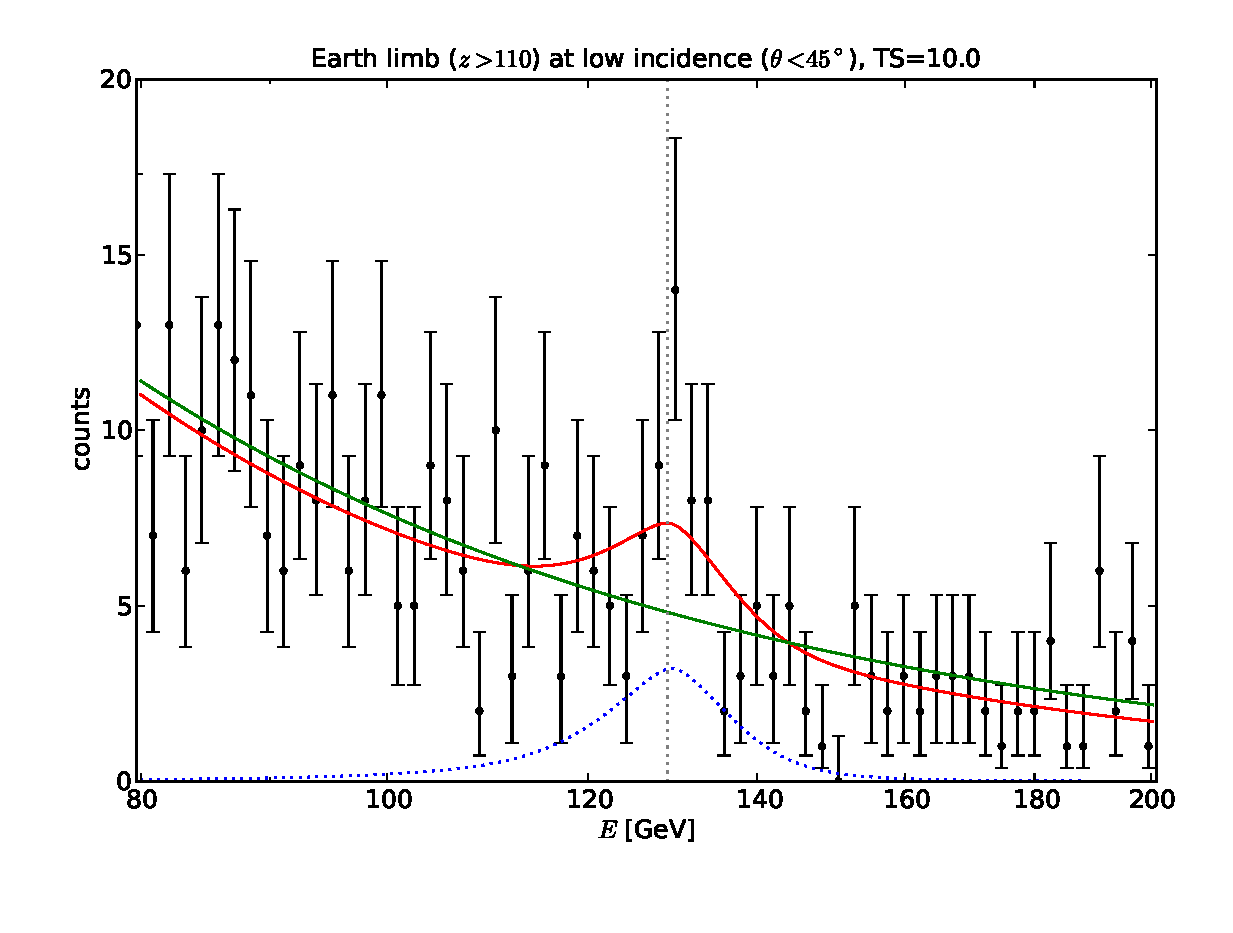
\includegraphics[width=0.48\linewidth]{plots/albedo_line_thetaCut.eps}
  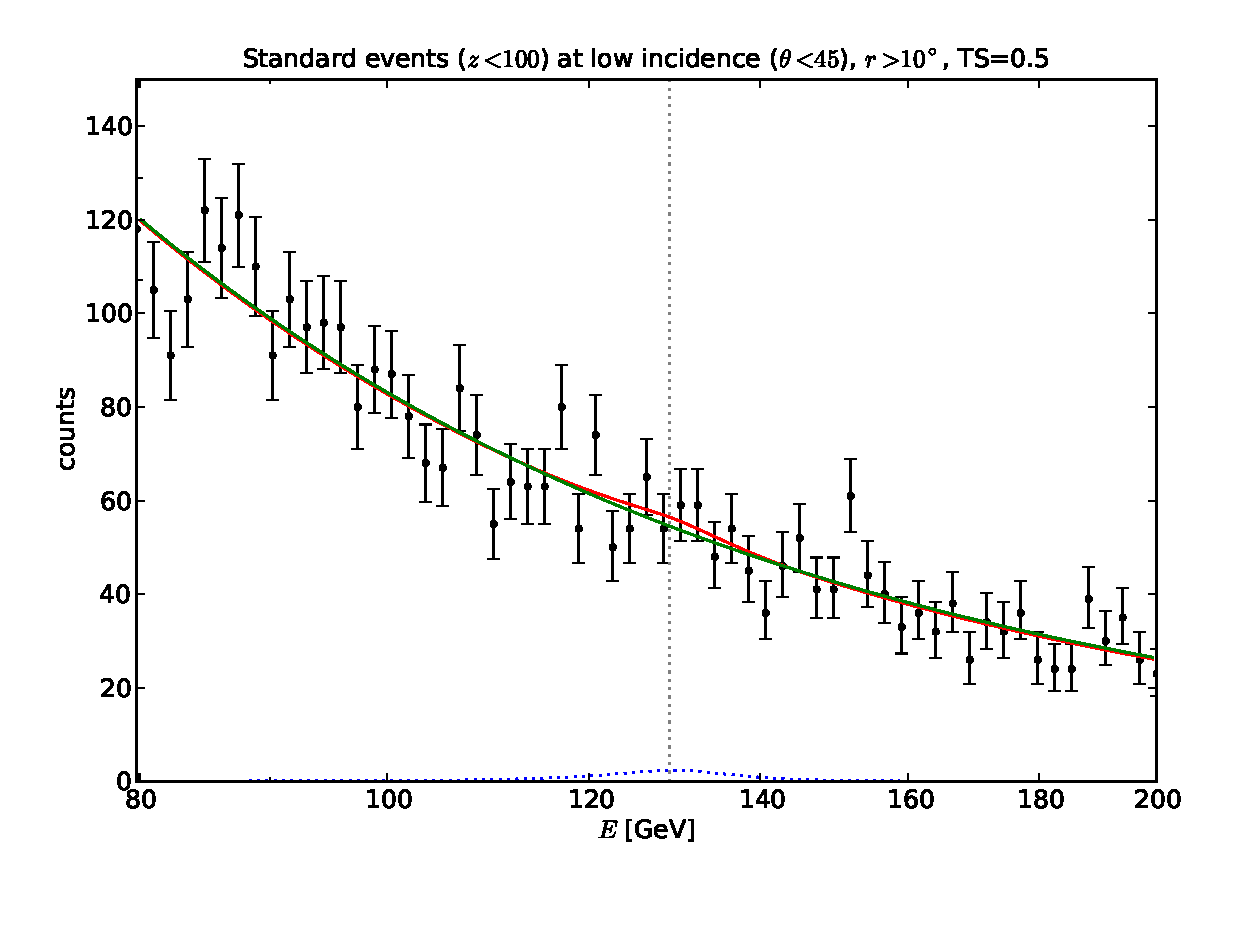
\includegraphics[width=0.48\linewidth]{plots/noalbedo_line_thetaCut.eps}
  \caption{\emph{Left panel:} Fit of a monochromatic line at 129 GeV to the
  low incidence angle Earth limb data. A 129 GeV line has a local significance of
  3.2$\sigma$.  \emph{Right panel:} same, but for the low incidence angle
  standard events. The inner $10^\circ$ around the Galactic center is masked
  out. We find no indication for a line at 129 GeV.}
  \label{fig:albedoline}
\end{figure*}

\begin{figure}[p]
  \centering
  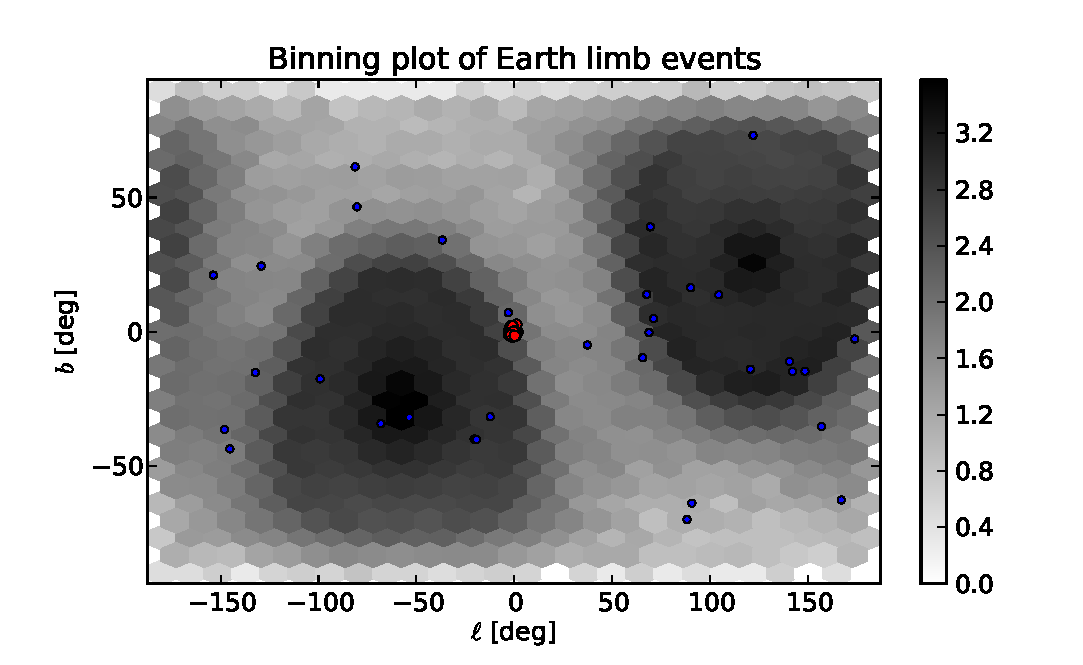
\includegraphics[width=1.0\linewidth]{plots/limb_l_b.eps}
  \caption{Same events, projected as an equal-area plot of Galactic $(\ell,
  \sin b)$.  The majority of high-incidence limb events appear near the
  orbital pole, which precesses around the celestial pole.  This pattern is
  expected from the observing strategy.}
  \label{fig:l-b}
\end{figure}

\begin{figure}[p]
  \begin{center}
    % \includegraphics{<+file+>}
    \fbox{\Huge Figure}
  \end{center}
  \caption{GC and limb events. Rocking angle vs. time.}
  \label{fig:rockTime}
\end{figure}

Now for some text...

Possible systematic errors:

- Extra events

{\bf Low energy photons:} Events would have to be mistakenly mapped from
either lower energy ($E \la 10$ GeV) gammas or much lower energy photons
(X-rays from the 1E $1740.7-2942$ microquasar?  511 keV photons?) in which the
Galactic center is much brighter.  It is difficult to see how this could
happen.

{\bf High energy photons:} At $E > 100$ GeV, the Galactic center is only
modestly brighter than the surrounding regions, so there are not enough
photons available.

{\bf Particle contamination:} If monochromatic photons from the limb are
difficult to explain, it is even harder to understand how mono-energetic
particles could be present. 

{\bf Effective area error:} An error in the LAT effective area (e.g. various
cuts are less restrictive for some reason) for $30\degree < \theta <
45\degree$ could explain the limb photons, but would also produce a line
everywhere in the Galactic plane.  No such line is seen outside of the GC. 

From these considerations, we conclude that there is no way for the limb line
to be caused by extra events. 

However, it is still plausible that there is a more subtle energy mapping
error that distorts the energy scale near 130 GeV.  In the next section, we
argue that this is a reasonable explanation of the limb line, but not of the
GC lines. 

\textbf{Mention Fig.~\ref{fig:GCevents}}

\begin{figure}[p]
  \centering
  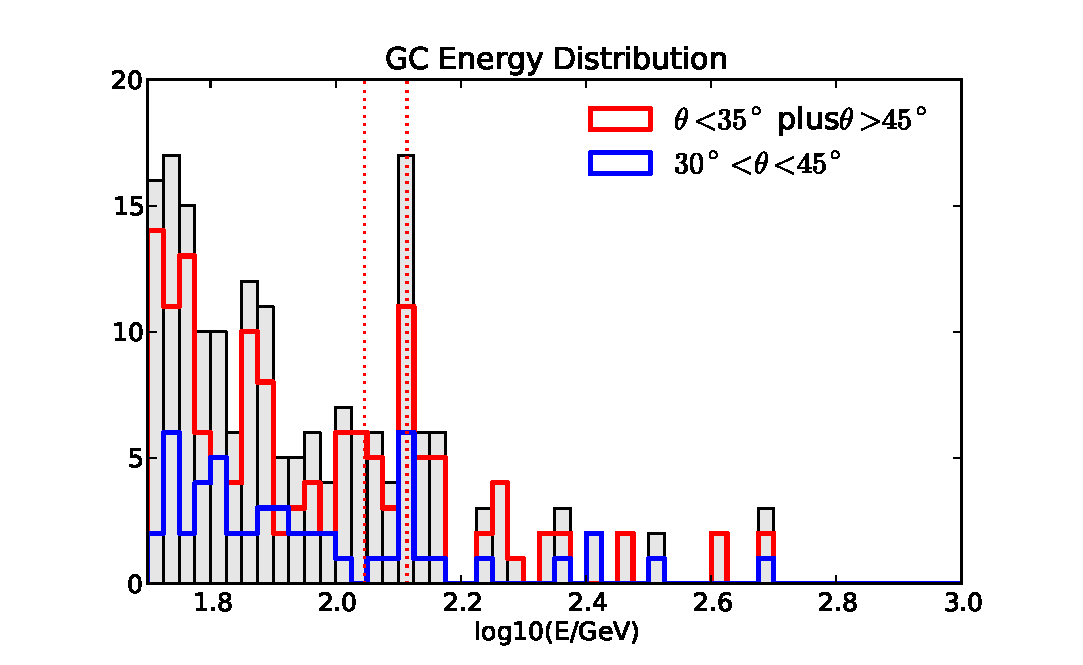
\includegraphics[width=1.0\linewidth]{plots/gc_energy.eps}
  \caption{Galactic center spectrum with with and without
  $30^\circ<\theta<45^\circ$ events.}
  \label{fig:GCevents}
\end{figure}



\clearpage

\section{Energy mapping error: a model for the limb bump}

\begin{figure}[p]
  \centering
  \includegraphics[width=1.0\linewidth]{plots/limb_bump_model.ps}
  \caption{Upper panel: function mapping true energy $E_t$ to reported energy
  $E$ (see Eqs. \ref{eq:yofx} and \ref{eq:dydx}).  Middle panel: The effect of
  this mapping on a spectrum of constant $dN/d\log E_t$, as in Eq.
  \ref{eq:dndy} (red line) and also for mock data (black histogram).  Lower
  panel: Same, but for $dN/dE \sim E^{-2.6}$.  }
  \label{fig:bumpmodel}
\end{figure}

\begin{figure}[p]
\centering
\includegraphics[width=1.0\linewidth]{plots/limbfits.ps}
\caption{Fits of the energy mapping model to limb data for various ranges of
  inclination angle $\theta$.  The vertical dotted line corresponds to 130
  GeV.  The test statistic ($2\Delta\ln L$) for the best fit model (green
  line) relative to the null hypothesis (red line) is given, along with the
  significance, expressed in ``sigma'' including a penalty for the 3
  additional degrees of freedom.  The deviation from linearity is only
  significant in the $30\degree < \theta < 45\degree$ panel.}
\label{fig:limbfits}
\end{figure}

Given the difficulty in explaining the excess any other way, we consider the
possibility that the limb bump results from an energy mapping error.  We
propose a simple model, in which the mapping from true energy to reported
energy, $E(E_t)$, is linear except for a bump near some reference energy.
Smooth low-level perturbations over large energy scales are not relevant here,
and could be absorbed in the effective area calibration.  In order to include
a small-scale bump in the response, we introduce a local compact perturbation
in the form of a Gaussian.  It is convenient to work in logarithmic
quantities, so we take $x=\log E_t, y=\log E$, and
\be
\label{eq:yofx}
y=x - A\sigma \exp\left(\frac{1}{2}-\frac{(x-x_0)^2}{2\sigma^2}\right),
\ee
where $A$ is a dimensionless amplitude of the bump ($-1<A<1$ is required
for monotonicity of $y(x)$), $x_0$ is a reference energy, and $\sigma$ is the
width of the bump (see Figure \ref{fig:bumpmodel}).
The effect of the distortion is to change the true spectrum $dN/dx =
dN/dlog(E_t)$ into an observed spectrum
\be
\label{eq:dndy}
\frac{dN}{dy} = \frac{dN}{dx} \left(\frac{dy}{dx}\right)^{-1} ,
\ee
with
\be
\label{eq:dydx}
\frac{dy}{dx} = 1 + A\sigma \exp\left(\frac{1}{2}-\frac{(x-x_0)^2}{2\sigma^2}\right)
\frac{x-x_0}{\sigma^2}.
\ee
Note that that the extreme values of $dy/dx = 1 \pm A$ occur at $x-x_0 = \pm
\sigma$ and at $y=x_0(\pm1-A)\sigma$.  Assuming the true limb spectrum is a
power law, we may apply this factor to obtain a model spectrum, and maximize
the Poisson likelihood of observing the data given the model.

To illustrate that this model can generate a spectrum similar to the limb bump
spectrum, we show 10 random realizations of a $dN/dE \sim E^{-2.6}$ spectrum
with this distortion in Figure \ref{fig:bumpmodelmany}.
Some of these look very similar to the bump in Figure \ref{fig:Ehist-all}.


\clearpage
\section{Future}
Ways to progress.

One to two weeks of additional limb data would provide an exposure comparable
to the limb photons used here.  One option would be to release commissioning
data from early in the survey, if they are thought to be of sufficient
quality.  Otherwise, new limb observations could be undertaken, in order to
test the reality of the 130 GeV limb feature.  

If the 130 GeV feature is not replicated, it can be dismissed as a statistical
fluke.  If it reappears, a deeper investigation into its cause is warranted.  

Even then, it is a challenge to understand how such an instrumental feature
could be mapped so precisely onto a localized region within 5-10 degrees of
the GC.  The GC is not near the path of the orbital pole, nor its axis of
precession.  The orbital phase, precession, Earth's orbit, and time of year
are all well mixed by the few $\times10^4$ orbits and 25 precession cycles
over 1500 days.  We have shown that the events in question are drawn from
every part of event and spacecraft parameter space available in the public
files.  In the absence of any model of instrumental behavior that explains how
these events land near the GC and not elsewhere in the Galactic plane, it is
far fetched to say that they invalidate a result with a local significance of
$p\approx10^{-9}$.  


\section{Conclusions}

\clearpage
\appendix
\section{This here is an appendix}

Here are a bunch of plots that are good to have, and could have shown
something interesting, but do not. 

\begin{figure*}[p]
\centering
\includegraphics[width=0.45\textwidth]{plots/timehist.ps}
\caption{Time histogram (1-day bins) of suspicious limb events and all limb
events.  The suspicious events are only observed at high rocking
angles that occur during pointed observations.
}
\label{fig:timehist}
\end{figure*}


\begin{figure*}[p]
\centering
\includegraphics[width=0.45\textwidth]{plots/Ehist-frontback.ps}
\caption{Energy histogram as in Figure \ref{fig:Ehist-all}, but for front
  (upper panel) and back (lower panel) converting events.  The 130 GeV excess
  appears equally in front and back converting events. 
}
\label{fig:Ehist-frontback}
\end{figure*}



\begin{figure*}[p]
\centering
\includegraphics[width=0.45\textwidth]{plots/theta-E-frontback.ps}
\caption{Same as ??? but for front and back converting events.}
\label{fig:theta-E-frontback}
\end{figure*}

\begin{figure*}[p]
\centering
\includegraphics[width=0.45\textwidth]{plots/geo-lonlat.ps}
\caption{Distribution of suspicious events in Earth longitude and latitude
(upper panel) and satellite zenith RA,dec (lower panel).   The
avoidance of the SAA leaves a hole in the upper panel.}
\label{fig:geo-lonlat}
\end{figure*}

\begin{figure*}[p]
\centering
\includegraphics[width=0.45\textwidth]{plots/spacecraft-zx.ps}
\caption{Direction of spacecraft Z axis (boresight direction) and X axis
(Solar panel direction) for the suspicious events.
}
\label{fig:spacecraft-zx}
\end{figure*}

\begin{figure*}[p]
\centering
\includegraphics[width=0.45\textwidth]{plots/earth-az.ps}
\caption{Zenith angle vs. Earth azimuth angle for limb photons.  As expected,
  the $\theta > 60\degree$ limb photons observed in survey mode are seen
  predominantly to the north and south azimuth directions, i.e approximately
  perpendicular to the orbit direction.  }
\label{fig:earth-az}
\end{figure*}

\begin{figure*}[p]
\centering
\includegraphics[width=0.45\textwidth]{plots/sun.ps}
\caption{Blue, red, and black events as a function of orbital precession phase
  (upper panel) and time of year (lower panel).  Note that there are only
  about 6 months of the year during which the 38 limb events are seen. 
}
\label{fig:sun}
\end{figure*}

\begin{figure*}[p]
  \centering
  \includegraphics[width=0.6\textwidth]{plots/limb_bump_model_many.ps}
  \caption{Ten mock spectra of an underlying spectrum $dN/dE \sim E^{-2.6}$,
  distorted according to Eq. \ref{eq:dndy}.  Note the similarity to the
  $30\degree < \theta < 45\degree$ panel in Figure \ref{fig:Ehist-all}.  }
  \label{fig:bumpmodelmany}
\end{figure*}
 
\begin{figure*}[p]
  \centering
  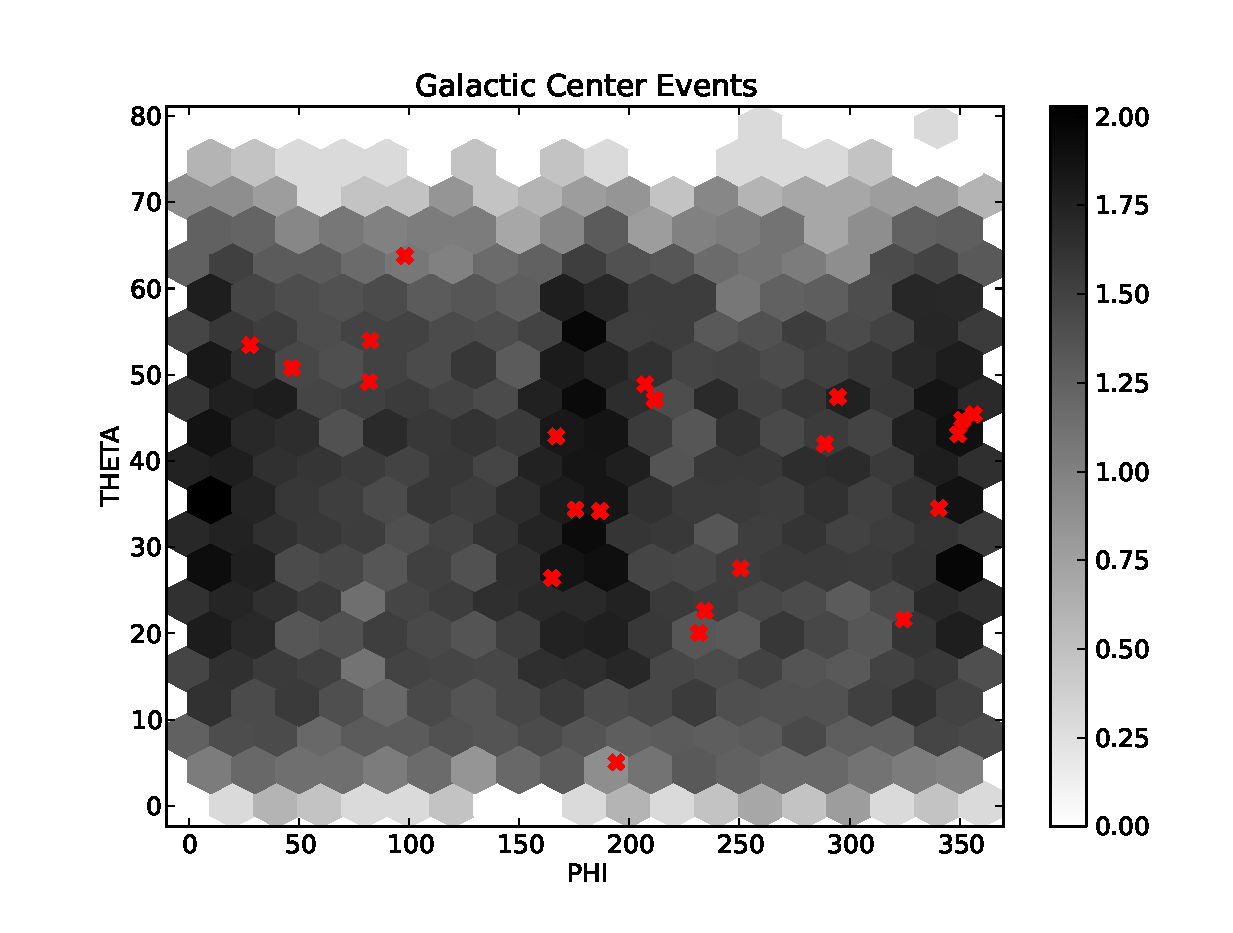
\includegraphics[width=0.48\textwidth]{plots/gc_theta_phi.eps}
  \includegraphics[width=0.48\textwidth]{plots/limb_theta_phi.eps}
  \caption{Line events (125 GeV $< E <$ 140 GeV) in physical detector angle
  coordinates ($\theta, \phi$).  The $30\degree < \theta < 45\degree$ events
  are blue in this and following panels}
  \label{fig:theta-phi}
\end{figure*}

\begin{figure}[p]
  \centering
  \includegraphics[width=0.9\linewidth]{plots/rockangle.ps}
  \caption{Rock angle -- \textbf{need to add red and blue to this plot}...  }
  \label{fig:rock}
\end{figure}


\bibliography{systematics}

\end{document}
